% Options for packages loaded elsewhere
\PassOptionsToPackage{unicode}{hyperref}
\PassOptionsToPackage{hyphens}{url}
%
\documentclass[
  12,
]{article}
\usepackage{lmodern}
\usepackage{amssymb,amsmath}
\usepackage{ifxetex,ifluatex}
\ifnum 0\ifxetex 1\fi\ifluatex 1\fi=0 % if pdftex
  \usepackage[T1]{fontenc}
  \usepackage[utf8]{inputenc}
  \usepackage{textcomp} % provide euro and other symbols
\else % if luatex or xetex
  \usepackage{unicode-math}
  \defaultfontfeatures{Scale=MatchLowercase}
  \defaultfontfeatures[\rmfamily]{Ligatures=TeX,Scale=1}
\fi
% Use upquote if available, for straight quotes in verbatim environments
\IfFileExists{upquote.sty}{\usepackage{upquote}}{}
\IfFileExists{microtype.sty}{% use microtype if available
  \usepackage[]{microtype}
  \UseMicrotypeSet[protrusion]{basicmath} % disable protrusion for tt fonts
}{}
\makeatletter
\@ifundefined{KOMAClassName}{% if non-KOMA class
  \IfFileExists{parskip.sty}{%
    \usepackage{parskip}
  }{% else
    \setlength{\parindent}{0pt}
    \setlength{\parskip}{6pt plus 2pt minus 1pt}}
}{% if KOMA class
  \KOMAoptions{parskip=half}}
\makeatother
\usepackage{xcolor}
\IfFileExists{xurl.sty}{\usepackage{xurl}}{} % add URL line breaks if available
\IfFileExists{bookmark.sty}{\usepackage{bookmark}}{\usepackage{hyperref}}
\hypersetup{
  pdftitle={Diplomatura en análisis de datos aplicados al desarrollo de políticas públicas - Grupo 4 Trabajo Final},
  pdfauthor={Emilio Madias, Gustavo Merino, Silvia Palacios},
  hidelinks,
  pdfcreator={LaTeX via pandoc}}
\urlstyle{same} % disable monospaced font for URLs
\usepackage[margin=1in]{geometry}
\usepackage{longtable,booktabs}
% Correct order of tables after \paragraph or \subparagraph
\usepackage{etoolbox}
\makeatletter
\patchcmd\longtable{\par}{\if@noskipsec\mbox{}\fi\par}{}{}
\makeatother
% Allow footnotes in longtable head/foot
\IfFileExists{footnotehyper.sty}{\usepackage{footnotehyper}}{\usepackage{footnote}}
\makesavenoteenv{longtable}
\usepackage{graphicx,grffile}
\makeatletter
\def\maxwidth{\ifdim\Gin@nat@width>\linewidth\linewidth\else\Gin@nat@width\fi}
\def\maxheight{\ifdim\Gin@nat@height>\textheight\textheight\else\Gin@nat@height\fi}
\makeatother
% Scale images if necessary, so that they will not overflow the page
% margins by default, and it is still possible to overwrite the defaults
% using explicit options in \includegraphics[width, height, ...]{}
\setkeys{Gin}{width=\maxwidth,height=\maxheight,keepaspectratio}
% Set default figure placement to htbp
\makeatletter
\def\fps@figure{htbp}
\makeatother
\setlength{\emergencystretch}{3em} % prevent overfull lines
\providecommand{\tightlist}{%
  \setlength{\itemsep}{0pt}\setlength{\parskip}{0pt}}
\setcounter{secnumdepth}{-\maxdimen} % remove section numbering

\title{Diplomatura en análisis de datos aplicados al desarrollo de políticas
públicas - Grupo 4 Trabajo Final}
\author{Emilio Madias, Gustavo Merino, Silvia Palacios}
\date{9/7/2021}

\begin{document}
\maketitle

\hypertarget{anuxe1lisis-presupuestario-y-de-beneficiarios-de-asignaciuxf3n-universal-por-hijo-auh-en-un-peruxedodo-de-7-auxf1os-2013-2020}{%
\section{Análisis Presupuestario y de Beneficiarios de Asignación
Universal Por Hijo (AUH) en un período de 7 años
(2013-2020)}\label{anuxe1lisis-presupuestario-y-de-beneficiarios-de-asignaciuxf3n-universal-por-hijo-auh-en-un-peruxedodo-de-7-auxf1os-2013-2020}}

\hypertarget{objetivo-analizar-la-implementaciuxf3n-de-la-poluxedtica-puxfablica-de-la-auh-desde-un-aspecto-cuantitativo-y-cualitativo-en-un-periodo-de-7-auxf1os-2013-2020}{%
\subsection{Objetivo: Analizar la implementación de la política pública
de la AUH desde un aspecto cuantitativo y cualitativo en un periodo de 7
años
(2013-2020)}\label{objetivo-analizar-la-implementaciuxf3n-de-la-poluxedtica-puxfablica-de-la-auh-desde-un-aspecto-cuantitativo-y-cualitativo-en-un-periodo-de-7-auxf1os-2013-2020}}

Desde su implementación, la Asignación Universal Por Hijo (llamada
también Asignación Universal para Protección Social) ha sido una
política pública que pretende fortalecer la protección social de
sectores que están marginados de otras políticas por carecer de empleo o
pertenecer a población con empleo informal o inestable.

Este estudio pretende realizar un análisis reproducible de dicha
política pública tanto desde el punto de vista de su asignación
presupuestaria así como la caracterización de sus beneficiarios

El carácter de reproducible está dado a partir de que para su
realización se utilizarán datos abiertos que son publicados por
distintos organismos públicos.

\hypertarget{datasets-utilizados}{%
\subsection{\texorpdfstring{\textcolor{darkblue}{Datasets
utilizados}}{Datasets utilizados}}\label{datasets-utilizados}}

Los datos abiertos que tomaremos son:

\begin{itemize}
\item
  de Presupuesto Nacional (Presupuesto de gastos y su ejecución
  detallada - agrupación anual)
  \url{https://www.presupuestoabierto.gob.ar/sici/datos-abiertos}
\item
  de Anses (Estadísticas de la Seguridad Social)
  \url{https://www.anses.gob.ar/institucional/datos-abiertos}
\item
  de Indec (Proyección de población)
  \url{https://www.indec.gob.ar/indec/web/Nivel4-Tema-2-24-84}
\end{itemize}

\hypertarget{aspectos-tuxe9cnicos}{%
\subsection{\texorpdfstring{\textcolor{darkblue}{Aspectos
técnicos}}{Aspectos técnicos}}\label{aspectos-tuxe9cnicos}}

Este análisis se realizó utilizando

\textcolor{pink}{\textbf{R para limpiar y analizar los datos}}

\textcolor{pink}{\textbf{R Markdown para presentar el informe}}

\textcolor{pink}{\textbf{Visualizaciones en R para graficar los
hallazgos}}

El software utilizado para la codificación fue RStudio

\hypertarget{introducciuxf3n}{%
\subsection{\texorpdfstring{\textcolor{darkblue}{Introducción}}{Introducción}}\label{introducciuxf3n}}

\hypertarget{marco-teuxf3rico-y-antecedentes-histuxf3ricos}{%
\subsubsection{Marco teórico y antecedentes
históricos}\label{marco-teuxf3rico-y-antecedentes-histuxf3ricos}}

La Asignación Universal por Hijo (AUH) fue creada en el año 2009
mediante el Decreto 1602/2009 que incorpora la AUH al régimen de
asignaciones familiares dentro del alcance de la ley 24.714. Nace como
un instrumento de protección social se enmarca en el contexto de
derechos económicos, sociales y culturales, que constituyen una amplia
categoría de derechos humanos, garantizados en tratados internacionales
y regionales para proteger a los individuos ante determinados riesgos
como la vejez, el desempleo, la invalidez y por sobre todo, la pobreza.

En el censo nacional de 2010 se registraron 14 millones de niños y
adolescentes menores de 19 años.

La AUH se crea como una extensión del Régimen de Asignación Familiares
tanto para los subsistemas contributivo como no contributivo
incorporando como beneficiarios a los hijos de trabajadores no
registrados en el sistema de seguridad social y a trabajadores
desocupados que no cobran el seguro de desempleo. Esta medida está
incluida en las políticas públicas para protección social que pretende
mejorar la calidad de vida de los sectores relegados dentro de la
informalidad laboral, pretendiendo brindar un apoyo económico que igual
a todos los niños más allá de la situación laboral de sus padres y
generando mejoras en las familias de menos ingresos de la población.

Dentro de las políticas públicas, la implementación de AUH es un intento
de acercar un beneficio directamente a la población que se encuentra en
una situación de mayor vulnerabilidad, en el corto plazo y de manera
continua, aunque también contempla una meta final de largo plazo dado
que plantea detener la dinámica de la pobreza intergeneracional. Su
implementación además, persigue otros objetivos vinculados a las
distintas esferas del desarrollo infantil, creando una retroalimentación
entre el aumento en el poder adquisitivo del hogar pretendiendo una
mejora en la alimentación, el acceso a la educación y la salud. A través
de su implementación se fortalece el ejercicio de los derechos del niño
incluidos en la ley 26061 del año 2005.

La protección a los derechos del niño a través de la AUH significa una
ayuda a favorecer la compra de materiales escolares, traslados y
vestimenta, para que los mismo puedan llevar adelante su escolaridad
disminuyendo el ausentismo. En el caso de los adolescentes, se pretende
minimizar el porcentaje de deserción escolar vinculada a la
participación de los menores en tareas productivas familiares o trabajo
que les permita aumentar el ingreso familiar. Es un beneficio de
carácter no retributivo que alcanza a todos los menores de 18 años cuyos
padres no se encuentren comprendidos en relaciones laborales formales ya
que estos últimos son beneficiarios de la asignación por hijo que es un
beneficio contributivo. Lo cobra sólo uno de los padres priorizando a la
mamá.

\hypertarget{destinatarios-y-requisitos}{%
\paragraph{Destinatarios y
requisitos}\label{destinatarios-y-requisitos}}

Los padres deben ser argentinos, residir en el país y tener DNI. Si son
extranjeros o naturalizados, tener 2 años de residencia y DNI. Los hijos
beneficiarios deben ser menores de 18 años, solteros y residir en el
país. Los hijos con discapacidad no tienen límite de edad. A partir de
2017 se incorpora al monotributista social, quedando conformados los
beneficiarios por los siguientes grupos:

\begin{itemize}
\item
  Personas desocupadas
\item
  Trabajadores en la economía informal con ingresos iguales o inferiores
  al salario mínimo, vital y móvil; que hoy es de \$ 25.920
\item
  Monotributistas sociales
\item
  Trabajadores del servicio doméstico
\item
  Quienes perciban alguno de los siguientes planes: Hacemos Futuro,
  Manos a la Obra y los programas del Ministerio de Trabajo.
\end{itemize}

Con esta inclusión se pretendió alcanzar la universalidad contemplando a
todos los niños por igual.

De esta manera a medida que sube el nivel de ingreso y/o la formalidad
en el empleo, baja la cobertura de la AUH y sube el de las asignaciones
familiares.

También se pretende fomentar tanto el cuidado de la salud como la
formación integral de los niños cuyos certificados de atención médica,
vacunación y escolaridad son obligatorios para la liquidación de la AUH.

Se paga mensualmente el 80\% de la asignación y una vez al año la
diferencia del 20\% de todos los meses, después de la presentación de
las obligaciones de salud y escolaridad mediante la Libreta de
Asignación Universal. El valor completo de la AUH general actualmente es
de \$ 4.504 y de \$ 14.677 para hijos con discapacidad. También hay un
valor adicional dependiendo de la zona de residencia.\footnote{Valores
  vigentes a junio 2021
  \url{https://www.anses.gob.ar/asignacion-universal-por-hijo}}

\begin{longtable}[]{@{}lll@{}}
\toprule
Asignación Familiar & General & Zona 1 ( 30\% + )\tabularnewline
\midrule
\endhead
Hijo & \$ 4504 & \$ 5856\tabularnewline
Hijo con discapacidad & \$ 14677 & \$ 19081\tabularnewline
Embarazo & \$ 4504 & \$ 5856\tabularnewline
Ayuda escolar anual & \$ 3776 & \$ 3776\tabularnewline
\bottomrule
\end{longtable}

General: Todo el país a excepción de las localidades comprendidas como
Zona 1

Zona 1: Provincias de La Pampa, Chubut, Neuquén, Río Negro, Santa Cruz,
Tierra del Fuego, Antártida e Islas del Atlántico Sur y el Partido de
Patagones, Pcia. de Buenos Aires

La AUH tiene un límite de cinco hijos por familia. Este límite del
quinto hijo no queda determinado el fundamento de por qué se estableció
de esa manera. Considerando que coexiste con las pensiones no
contributivas para madres de siete o más hijos, las familias con seis
hijos quedan en una situación de desprotección y desigualdad ante
aquellas familias de seis hijos de trabajadores asalariados formales.
Este punto nos plantea una inquietud sobre la inclusión del sexto hijo
en una futura actualización de la normativa vigente.

\hypertarget{asignaciuxf3n-por-embarazo}{%
\subparagraph{Asignación por
Embarazo}\label{asignaciuxf3n-por-embarazo}}

La llamada Asignación por embarazo para protección social que destinada
a:

\begin{itemize}
\item
  Mujeres desocupadas.
\item
  Trabajadoras informales con ingresos iguales o inferiores al Salario
  Mínimo, Vital y Móvil.
\item
  Monotributistas sociales.
\item
  Trabajadoras de servicio doméstico registradas.
\item
  Personas inscriptas en alguno de los programas Hacemos Futuro
  (Argentina Trabaja y Ellas Hacen), Manos a la Obra o Programas del
  Ministerio de Trabajo.
\end{itemize}

Las personas que se encuentren en alguna de las mencionadas situaciones
podrán acceder en la medida que su cónyuge o conviviente se encuentre
bajo la misma situación. Los requisitos para acceder son:

\begin{itemize}
\item
  Tener un embarazo de 12 semanas o más.
\item
  Cumplir con los controles médicos.
\item
  Ser argentina, residir en el país y tener DNI o extranjera o
  naturalizada, con 2 años de residencia en el país y DNI.
\item
  Ser trabajadora informal o desocupada inscripta en el Programa SUMAR y
  no tener obra social.
\end{itemize}

Se paga el 80\% mensualmente y el 20\% restante acumulando todos los
meses, al momento del nacimiento o interrupción del embarazo.

\hypertarget{otras-asignaciones-familiares}{%
\paragraph{Otras asignaciones
familiares}\label{otras-asignaciones-familiares}}

\hypertarget{asignaciuxf3n-familiar-por-hijo}{%
\subparagraph{Asignación Familiar por
Hijo}\label{asignaciuxf3n-familiar-por-hijo}}

La Asignación familiar por hijo se paga a los siguientes grupos de
beneficiarios:

\begin{itemize}
\tightlist
\item
  Trabajadores en relación de dependencia. (Sistema Único de
  Asignaciones Familiares - SUAF)
\item
  Trabajadores monotributistas.
\item
  Trabajadores de temporada con reserva de puesto de trabajo.
\item
  Trabajadores que se encuentren cobrando por una Aseguradora de Riesgos
  del Trabajo.
\item
  Trabajadores que cobren la Prestación por Desempleo.
\item
  Personas que cobren la Pensión Honorífica de Veteranos de Guerra del
  Atlántico Sur.
\item
  Jubilados y pensionados.
\end{itemize}

Para el pago de estas asignaciones se toma en cuenta el ``Ingreso del
Grupo Familiar'' (IGF) que consiste en la suma de todos los ingresos de
los integrantes del grupo familiar, el cual se calcula sumando los
siguientes ítems:

\begin{itemize}
\tightlist
\item
  las remuneraciones brutas y sumas no remunerativas declaradas por el
  empleador en el formulario 931 que presenta mensualmente en AFIP a los
  trabajadores en relación de dependencia, excluyendo las horas extras,
  el plus por zona desfavorable y el aguinaldo
\item
  más la Asignación Familiar por Maternidad / Maternidad Down (en caso
  de corresponder)
\item
  más las rentas de referencia para trabajadores autónomos,
  monotributistas y servicio doméstico
\item
  más los haberes de jubilación y pensión
\item
  más el monto de la Prestación por Desempleo
\item
  más Planes Sociales
\item
  más las sumas originadas en Prestaciones Contributivas y/o No
  Contributivas de cualquier índole
\end{itemize}

Si un integrante del grupo familiar percibe un importe bruto superior a
Pesos ciento cinco mil ciento treinta y nueve (\$ 105.139.-), se excluye
del cobro de asignaciones familiares al grupo familiar.{[}\^{}2{]}

Topes de Ingreso del Grupo Familiar Vigentes - Resolución ANSES Nº 51/21

\begin{itemize}
\tightlist
\item
  Tope Máximo de Ingreso del Grupo Familiar \$ 210.278
\item
  Tope Máximo de cada integrante del Grupo Familiar \$ 105.139
\end{itemize}

\textbf{Tabla Valores Asignación Familiar por Hijo (Ingreso por Grupo
Familiar)}

\begin{longtable}[]{@{}llllll@{}}
\toprule
Ingreso familiar & Zona normal & Zona 1 & Zona 2 & Zona 3 & Zona
4\tabularnewline
\midrule
\endhead
IGF hasta \$69.805 & \$4.504 & \$4.504 & \$9.719 & \$9.000 &
\$9.719\tabularnewline
IGF entre \$69.805,01 y \$102.377 & \$3.038 & \$4.013 & \$6.013 &
\$7.997 & \$7.997\tabularnewline
IGF entre \$102.377,01 y \$118.199 & \$1.836 & \$3.616 & \$5.429 &
\$7.226 & \$7.226\tabularnewline
IGF entre \$118.199,01 y \$210.278 & \$945 & \$1.852 & \$2.774 & \$3.671
& \$3.671\tabularnewline
\bottomrule
\end{longtable}

{[}\^{}2{]} Valores vigentes a junio 2021
\url{https://www.anses.gob.ar/asignacion-familiar-por-hijo}

Las diferentes zonas geográficas tienen incremento según tabla de grupos

\begin{itemize}
\item
  Zona 1: Neuquén, La Pampa, Río Negro; Departamentos Bermejo, Ramón
  Lista y Matacos en Formosa; Departamento Las Heras (Distrito Las
  Cuevas); Departamento Luján de Cuyo(Distrito Potrerillos, Carrizal,
  Agrelo, Ugarteche, Perdriel, Las Compuertas); Departamento Tupungato
  (Distritos Santa Clara, Zapata, San José, Anchoris); Departamento
  Tunuyan (Distrito Los Arboles, Los Chacayes, Campo de los Andes);
  Departamento San Carlos (Distrito Pareditas); Departamento San Rafael
  (Distrito Cuadro Benegas); Departamento Malargüe (Distritos Malargüe,
  Río Grande, Río Barrancas, Agua Escondida) Departamento Maipú
  (Distritos Rusell, Cruz de Piedra, Lumlunta, Las Barrancas);
  Departamento Rivadavia (Distritos El Mirador, Los Campamentos, Los
  Arboles, Reducción, Medrano) en Mendoza; Orán (excepto la ciudad de
  San Ramon de la Nueva Oran y su ejido urbano) en Salta
\item
  Zona 2: Pcia. de Chubut
\item
  Zona 3: Departamentos Antofagasta de la Sierra (actividad minera) en
  Catamarca; Departamentos Cochinoca, Humahuaca, Rinconada, Santa
  Catalina, Susques, Yavi en Jujuy; Departamentos Los Andes, Santa
  Victoria, Rivadavia y Grl San Martin (excepto la ciudad de Tartagal y
  su ejido urbano) en Salta
\item
  Zona 4: Pcias. de Tierra del Fuego, Santa Cruz e Islas del Atlántico
  Sur
\end{itemize}

\textbf{Asignación por Hijo para Monotributistas}

\begin{longtable}[]{@{}llllll@{}}
\toprule
Asignación Familiar & A,B,C,D & E y F & G & H & I,J,K\tabularnewline
\midrule
\endhead
Prenatal & \$ 4504 & \$ 3038 & \$ 1836 & \$ 945 & \$ 0\tabularnewline
Hijo & \$ 4504 & \$ 3038 & \$ 1836 & \$ 945 & \$ 0\tabularnewline
Hijo con discapacidad & \$ 14677 & \$ 10381 & \$ 6552 & \$ 6552 & \$
6552\tabularnewline
\bottomrule
\end{longtable}

Valores vigentes a junio 2021
\url{https://www.anses.gob.ar/asignacion-familiar-por-hijo}

\hypertarget{enfoque-presupuestario}{%
\subsubsection{Enfoque presupuestario}\label{enfoque-presupuestario}}

La asignación universal por hijo (identificada en el presupuesto como
asignación universal para protección social) es una política que, si
bien se extiende a todo el país, es financiada íntegramente por el
Estado Nacional. Los fondos destinados para su ejecución están incluidos
anualmente en la Ley de Presupuesto, la cual es sancionada por el
Congreso Nacional generalmente en los meses de diciembre de cada año. El
organismo que se encarga de la formulación y ejecución de esta política
es la Administración Nacional de Seguridad Social (ANSES). Este
organismo fue creado en 1991 a través del Decreto N° 2.741/91, es un
organismo descentralizado que desarrolla sus funciones en el ámbito del
Ministerio de Trabajo, Empleo y Seguridad Social (MTESS). Sin embargo,
durante parte del periodo estudiado la ANSES depende del Ministerio de
Desarrollo Social debido a la transformación del Ministerio de Trabajo
en la Secretaría de Gobierno de Trabajo que dependía del Ministerio de
Desarrollo Social. ANSES tiene a su cargo la administración de las
prestaciones y los servicios de la Seguridad Social en la República
Argentina. Asimismo, desde la vigencia del Decreto N° 897/07 ANSeS es
responsable de la administración del Fondo de Garantía de
Sustentabilidad (FGS) del Sistema Integrado Previsional Argentino
(SIPA).

Dentro del esquema de programas presupuestarios del ANSES la política
que estudiamos se encuentra dentro del Programa 19 ``Asignaciones
Familiares'' cuya Unidad Ejecutora es la ``Subdirección Ejecutiva de
Prestaciones''

Este programa tiene a su cargo el pago de:

\begin{itemize}
\item
  las asignaciones familiares correspondientes a trabajadores en
  relación de dependencia del sector privado y del Sector Público
  Nacional, de los beneficiarios de la Ley sobre Riesgos de Trabajo, del
  Seguro de Desempleo y del Sistema Integrado Previsional Argentino,
  según lo dispuesto por la Ley Nº 24.714 y sus modificatorias
\item
  las asignaciones universales por hijo y embarazo que por los Decretos
  Nº 1.602/09 y Nº 446/11 se incorporan como inciso c) del art.1º de la
  citada Ley.
\item
  Se incluyen también las asignaciones familiares derivadas de los
  beneficios de la Pensión Universal para el Adulto Mayor; de Pensiones
  no Contributivas y las de inscriptos al monotributo
\end{itemize}

Los montos asignados en la ley de Presupuesto, así como la descripción
de la política y sus metas físicas estimadas para cada año, se
encuentran detallados en
\url{https://www.economia.gob.ar/onp/presupuestos/2021}

La ejecución presupuestaria se puede seguir en el sitio Presupuesto
Abierto \url{https://www.presupuestoabierto.gob.ar/sici/home}

\hypertarget{anuxe1lisis-presupuestario}{%
\subsection{\texorpdfstring{\textcolor{darkblue}{Análisis
Presupuestario}}{Análisis Presupuestario}}\label{anuxe1lisis-presupuestario}}

Para poder efectuar una comparación interanual de asignaciones
presupuestarias es necesario encontrar una unidad de medida que permita
dejar de lado el componente inflacionario que está presente en la
economía argentina.

La forma que elegimos es analizar desde el punto de vista de porcentaje
de participación sobre distintos conceptos de la economía.

En nuestro caso vamos a utilizar estos totalizadores:

\begin{itemize}
\item
  El PBI (Producto Bruto Interno)
\item
  El Gasto Total (Total ejecutado del Presupuesto Nacional al final de
  cada año)
\item
  El Gasto Social (Total ejecutado de la finalidad función 3 ``Servicios
  Sociales'' en el Presupuesto Nacional al final de cada año)
\end{itemize}

\hypertarget{anuxe1lisis-de-auh-respecto-al-pbi-al-gasto-total-y-al-gasto-social-del-presupuesto-nacional}{%
\subsubsection{Análisis de AUH respecto al PBI, al gasto total y al
gasto social del Presupuesto
Nacional}\label{anuxe1lisis-de-auh-respecto-al-pbi-al-gasto-total-y-al-gasto-social-del-presupuesto-nacional}}

Vamos a analizar gráficamente la evolución de la AUH como porcentaje del
PBI, del Gasto Total y del Gasto Social

Veremos en estos gráficos que la participación de la AUH en estos
indicadores es fluctuante y acompaña los períodos de la economía, en los
años de crisis el porcentaje sube y viceversa

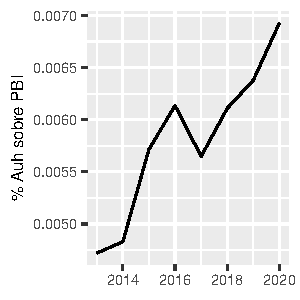
\includegraphics{Grupo4_Final_files/figure-latex/graficos_presu_1-1.pdf}
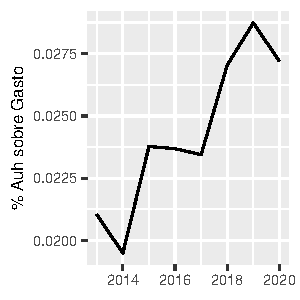
\includegraphics{Grupo4_Final_files/figure-latex/graficos_presu_1-2.pdf}
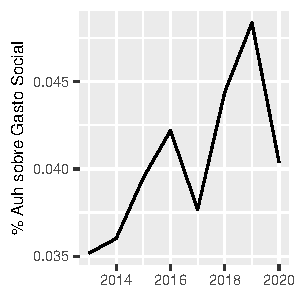
\includegraphics{Grupo4_Final_files/figure-latex/graficos_presu_1-3.pdf}

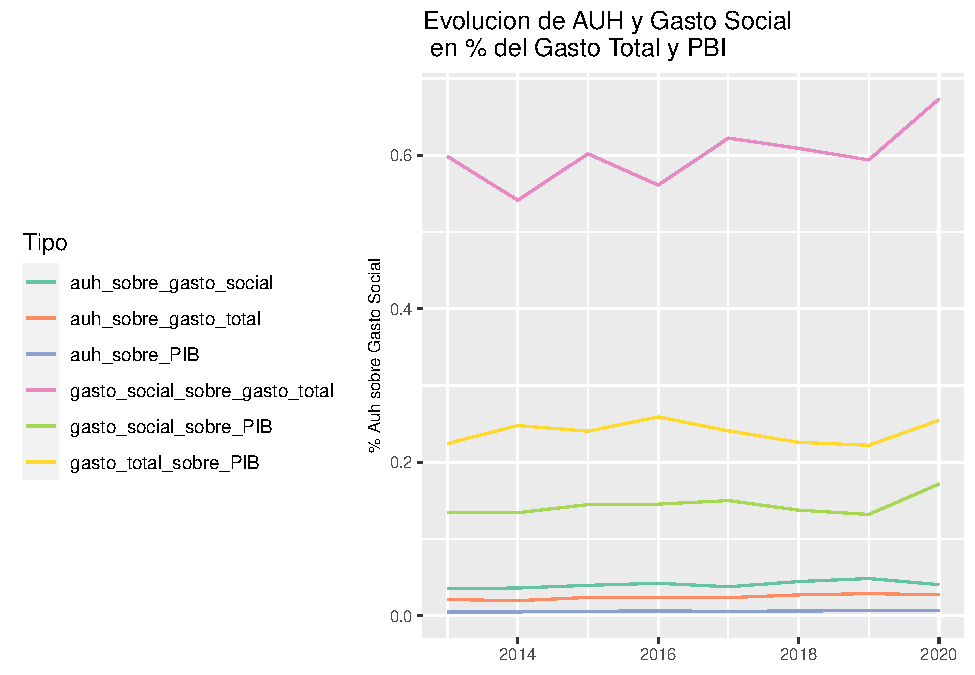
\includegraphics{Grupo4_Final_files/figure-latex/graficos_presu_11-1.pdf}

En este último gráfico analizamos el gasto social y la AUH respecto a
los demás indicadores. Así vemos la importancia que tiene el gasto
social sobre el gasto total (representa alrededor de un 60\% del mismo),
el \% del gasto total sobre el PBI (un poco más que 20\%) y en
consecuencia vemos que el gasto social contenido en el Presupuesto
Nacional representa un poco más del 10\% del PBI.

\hypertarget{alcance-del-presupuesto-nacional}{%
\paragraph{Alcance del Presupuesto
Nacional}\label{alcance-del-presupuesto-nacional}}

Es relevante recordar que el Presupuesto Nacional no representa todo el
Sector Público Nacional sino solo lo contemplado dentro de la Ley de
Presupuesto.

Lo vemos en este cuadro

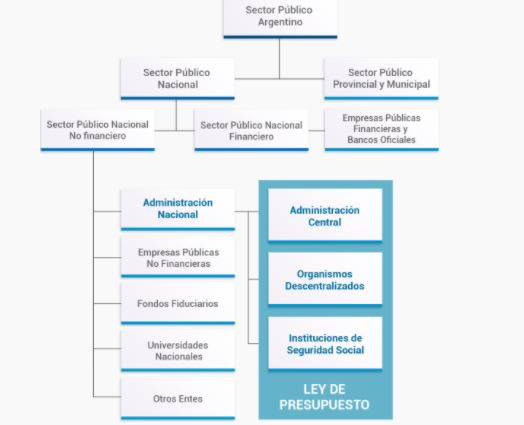
\includegraphics{Alcance_presupuesto.JPG}

Para más información acerca del alcance del Presupuesto consultar en
\url{https://www.presupuestoabierto.gob.ar/sici/que-incluye}

\hypertarget{anuxe1lisis-del-gasto-en-auh-respecto-a-otras-asignaciones-familiares-financiadas-por-anses}{%
\subsubsection{Análisis del gasto en AUH respecto a otras asignaciones
familiares financiadas por
ANSES}\label{anuxe1lisis-del-gasto-en-auh-respecto-a-otras-asignaciones-familiares-financiadas-por-anses}}

Ahora analizamos la AUH respecto a otras asignaciones familiares
financiadas por ANSES:

\begin{itemize}
\tightlist
\item
  Asignaciones Familiares Activos
\item
  Asignaciones Familiares Sector Público Nacional
\item
  Asignaciones Familiares Monotributistas
\item
  Asignaciones Familiares Pasivos
\item
  Asignaciones Familiares Pensión Universal
\end{itemize}

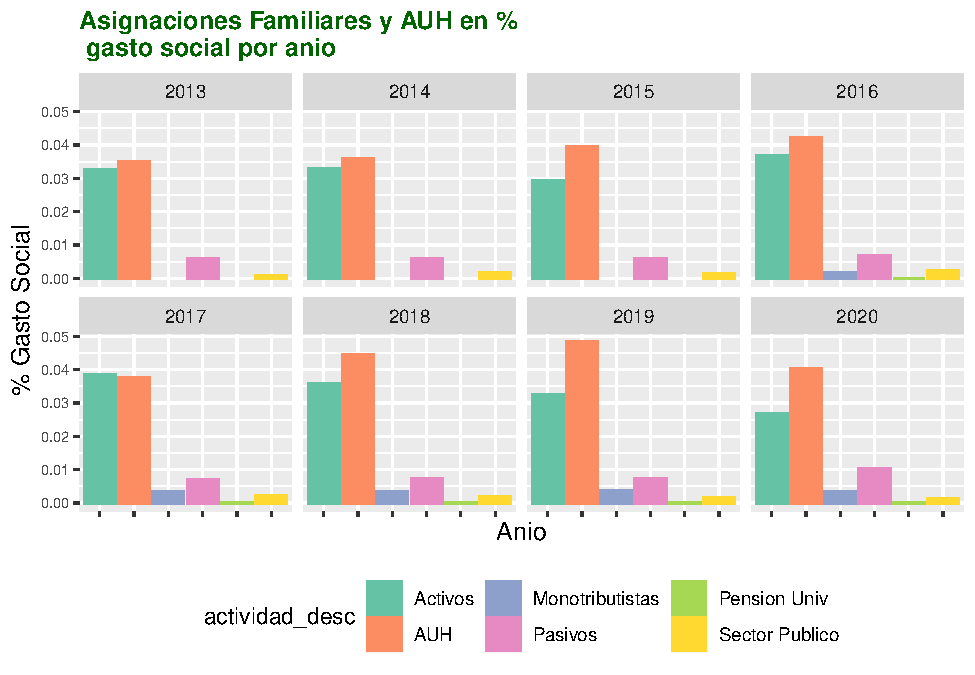
\includegraphics[width=0.8\linewidth]{Grupo4_Final_files/figure-latex/graficos_presu_2-1}
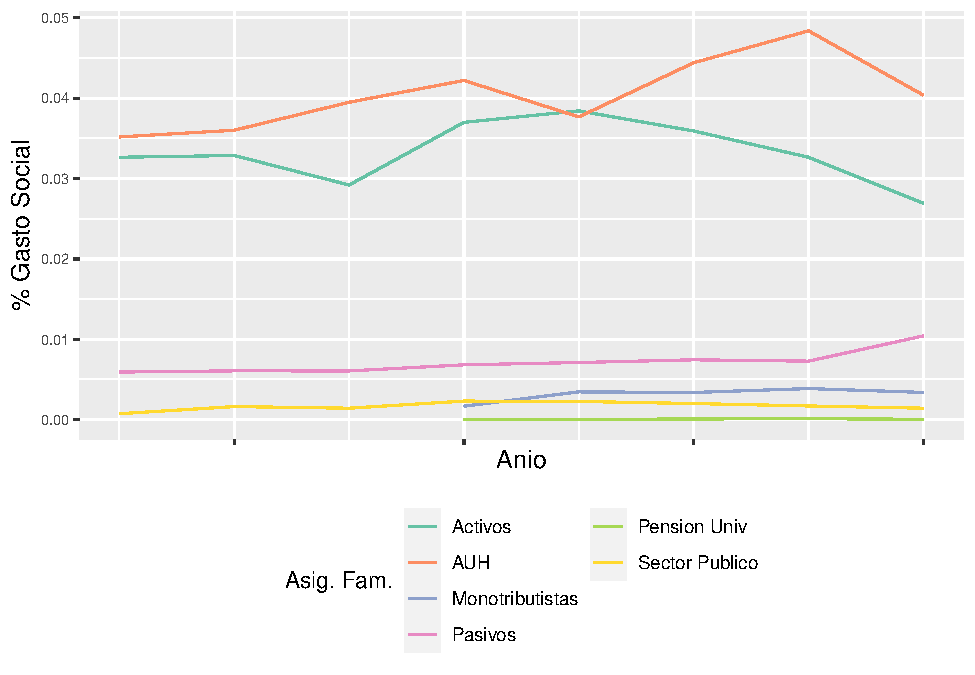
\includegraphics[width=0.8\linewidth]{Grupo4_Final_files/figure-latex/graficos_presu_2-2}

Es interesante ver que las asignaciones familiares a trabajadores
activos parecen tener una correlacion inversa con la AUH, cuando una
sube la otra baja. Y por otro lado vemos que con el correr de los años y
la crisis económica la AUH termina representando un monto mayor que la
asignación familiar a trabajadores activos.

\hypertarget{anuxe1lisis-de-la-auh-respecto-al-gasto-social-financiado-por-el-presupuesto-nacional}{%
\subsubsection{Análisis de la AUH respecto al Gasto Social financiado
por el Presupuesto
Nacional}\label{anuxe1lisis-de-la-auh-respecto-al-gasto-social-financiado-por-el-presupuesto-nacional}}

Para continuar con el análisis vamos a utilizar el clasificador
presupuestario por función. (llamado finalidad función)

Según el Manual de Clasificaciones Presupuestarias para el Sector
Público Nacional (disponible en
\url{https://capacitacion.mecon.gob.ar/manuales_nuevo/Presupuesto-Clasificador13.pdf}),
la clasificación funcional presenta el gasto público según la naturaleza
de los servicios que las instituciones públicas brindan a la comunidad.
Los gastos clasificados por finalidad y función permiten determinar los
objetivos generales y los medios a través de los cuales se estiman
alcanzar éstos. En estos términos la clasificación por finalidades y
funciones se constituye en un instrumento fundamental para la toma de
decisiones por el poder político.

La clasificación se divide en dos dígitos: el primero corresponde a la
finalidad y el segundo a la función

La lista completa es la siguiente:

\begin{itemize}
\tightlist
\item
  1 Administración gubernamental

  \begin{itemize}
  \tightlist
  \item
    1.1 Legislativa
  \item
    1.2 Judicial
  \item
    1.3 Dirección superior ejecutiva
  \item
    1.4 Relaciones exteriores
  \item
    1.5 Relaciones interiores
  \item
    1.6 Administración fiscal
  \item
    1.7 Control de la gestión pública
  \item
    1.8 Información y estadística básicas
  \end{itemize}
\item
  2 Servicios de defensa y seguridad

  \begin{itemize}
  \tightlist
  \item
    2.1 Defensa
  \item
    2.2 Seguridad interior
  \item
    2.3 Sistema penal
  \item
    2.4 Inteligencia
  \end{itemize}
\item
  3 Servicios sociales

  \begin{itemize}
  \tightlist
  \item
    3.1 Salud
  \item
    3.2 Promoción y asistencia social
  \item
    3.3 Seguridad social
  \item
    3.4 Educación y cultura
  \item
    3.5 Ciencia y técnica
  \item
    3.6 Trabajo
  \item
    3.7 Vivienda y urbanismo
  \item
    3.8 Agua potable y alcantarillado
  \item
    3.9 Otros servicios urbanos
  \end{itemize}
\item
  4 Servicios económicos

  \begin{itemize}
  \tightlist
  \item
    4.1 Energía, combustibles y minería
  \item
    4.2 Comunicaciones
  \item
    4.3 Transporte
  \item
    4.4 Ecología y medio ambiente
  \item
    4.5 Agricultura
  \item
    4.6 Industria
  \item
    4.7 Comercio, turismo y otros servicios
  \item
    4.8 Seguros y finanzas
  \end{itemize}
\item
  5 Deuda pública

  \begin{itemize}
  \tightlist
  \item
    5.1 Servicio de la deuda pública (intereses y gastos)
  \end{itemize}
\end{itemize}

La AUH pertenece a la finalidad ``Servicios Sociales'' (finalidad = 3) y
dentro de esa finalidad forma parte de la función ``Seguridad Social''
(3.3) (junto con otros gastos)

Realizamos ahora un análisis de cómo se compone el Gasto Social
(finalidad = 3) en cuanto a su distribución en sus distintas funciones

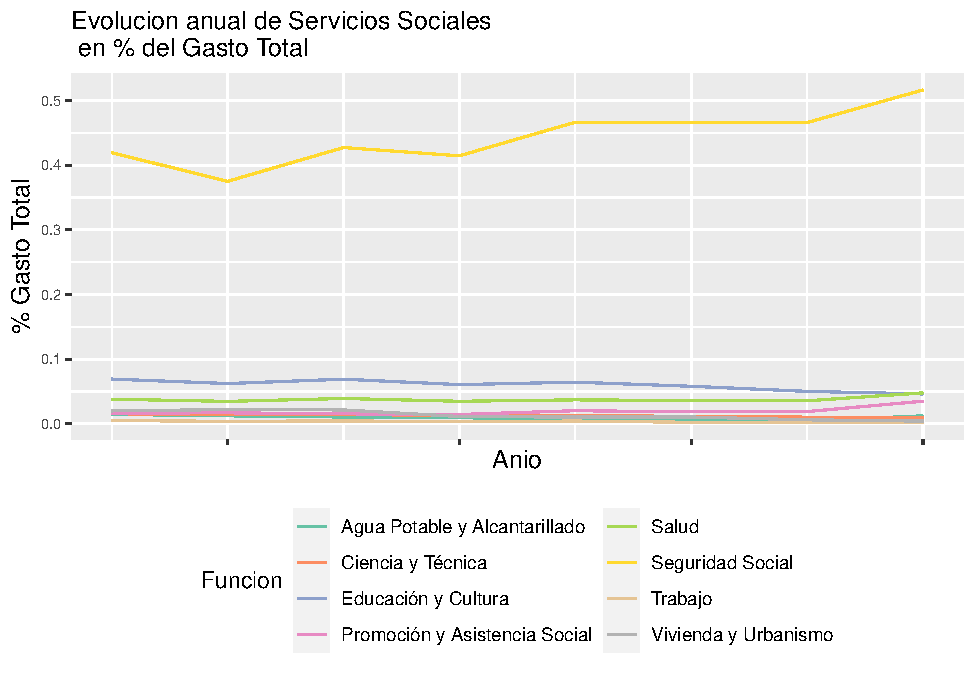
\includegraphics{Grupo4_Final_files/figure-latex/graficos_presu_3-1.pdf}

Como vemos en este gráfico el gasto en seguridad social explica gran
parte del gasto social.

Sin embargo, la mayor parte del gasto en Seguridad Social está dado por
las jubilaciones y pensiones. Por ello vamos a repetir el análisis pero
dejando solamente las asignaciones familiares en lugar de todo el gasto
en Seguridad Social

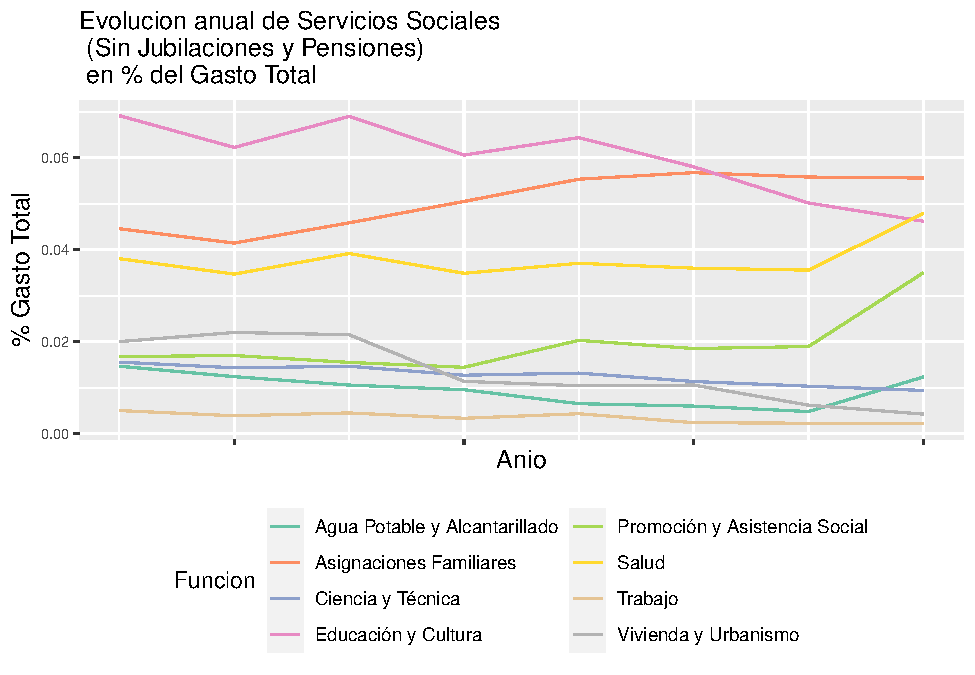
\includegraphics{Grupo4_Final_files/figure-latex/graficos_presu_4-1.pdf}

El mismo análisis pero dejando solo AUH en lugar de todas las
asignaciones familiares

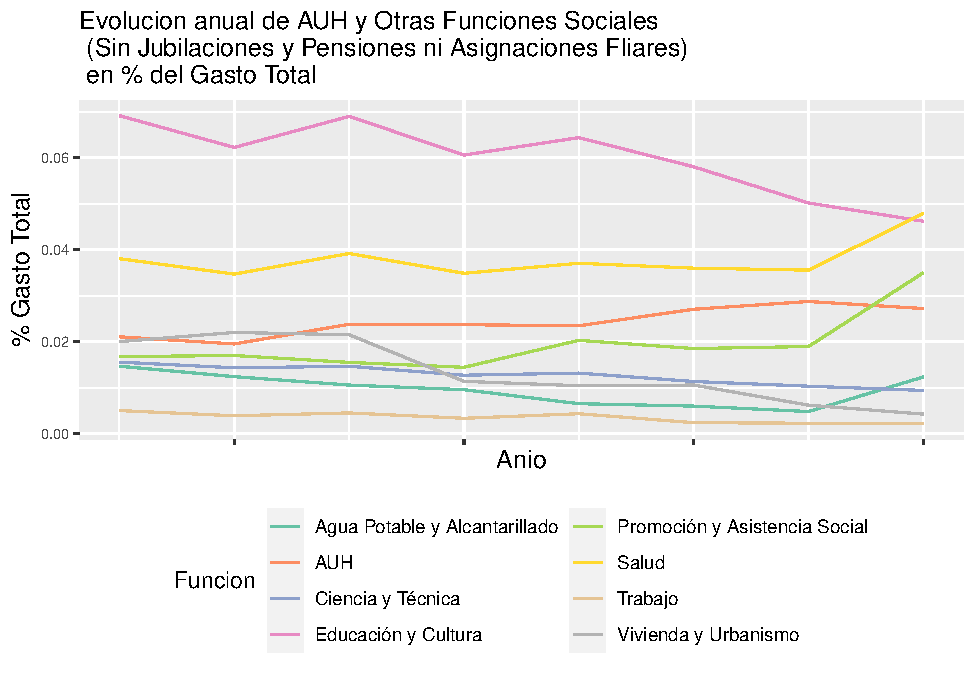
\includegraphics{Grupo4_Final_files/figure-latex/graficos_presu_5-1.pdf}

Como vemos la AUH es casi la única función que ha ido creciendo en su
peso respecto al gasto social. La mayoría de las demás funciones han
decaído salvo algunas que se mantienen relativamente constantes. En
2020, debido a la pandemia, se incrementaron los gastos en Salud

Por último, vamos a graficar cómo ha sido, en promedio la participación
de las asignaciones familiares y de la AUH respecto a las demás
funciones del gasto social a lo largo de los años del análisis

Presentamos dos gráficos, uno con todas las asignaciones familiares y
otro solo con la AUH

\begin{verbatim}
## [1] "Grafico de burbujas para graficar mejor la relacion entre asignaciones familiares y otros gastos sociales (sin Seguridad Social)"
\end{verbatim}

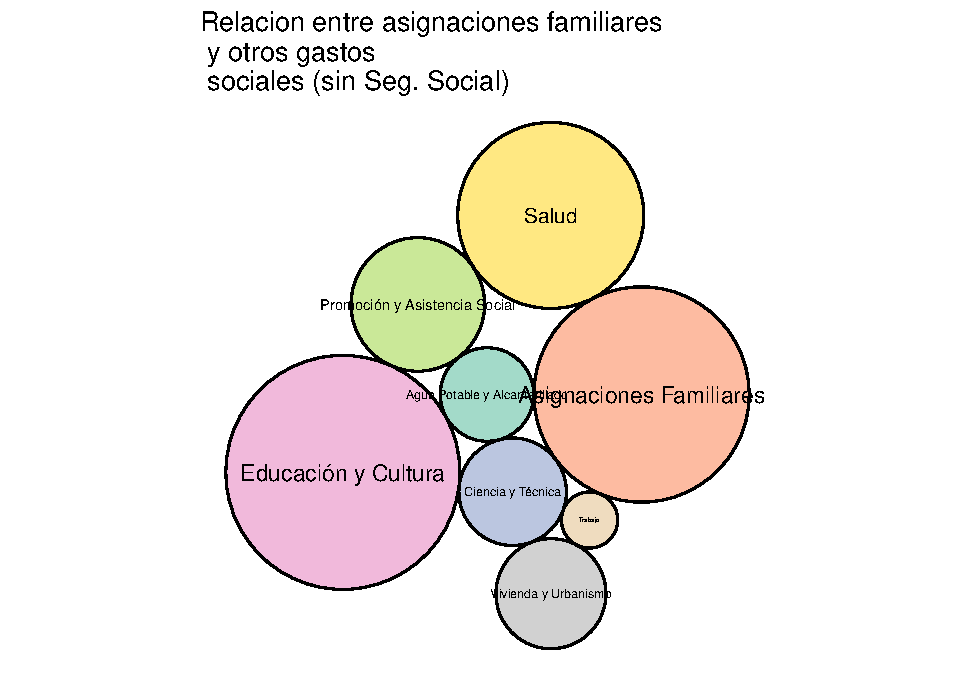
\includegraphics{Grupo4_Final_files/figure-latex/graficos_presu_6-1.pdf}

\begin{verbatim}
## [1] "Grafico de burbujas para graficar mejor relacion entre AUH y otros gastos sociales (sin Seguridad Social)"
\end{verbatim}

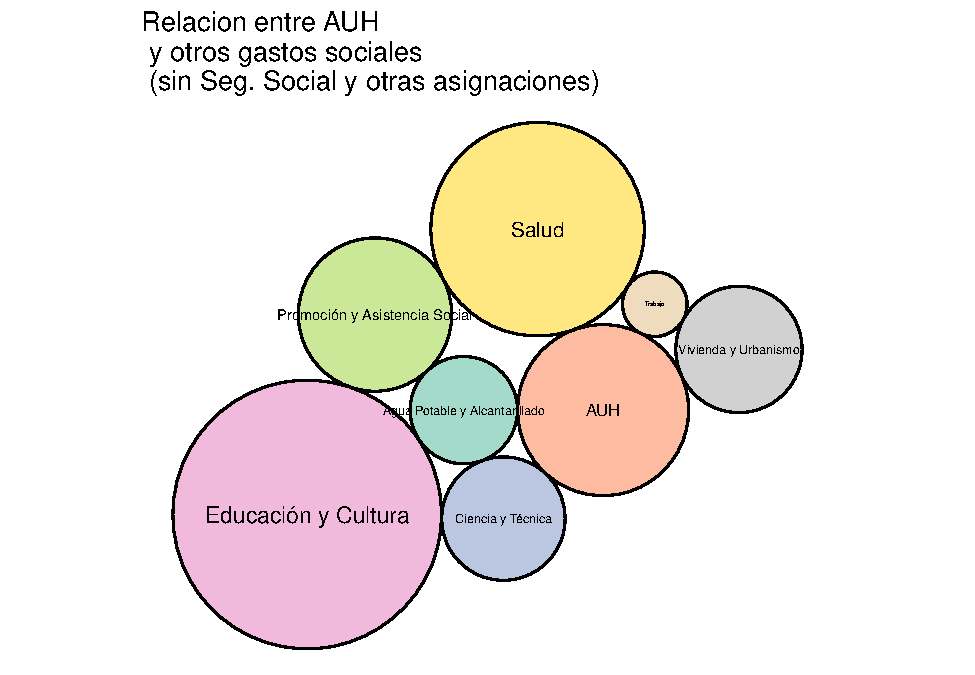
\includegraphics{Grupo4_Final_files/figure-latex/graficos_presu_6-2.pdf}

\hypertarget{anuxe1lisis-datos-anses}{%
\subsubsection{Análisis Datos ANSES}\label{anuxe1lisis-datos-anses}}

Aquí vemos el dataset de Anses desagregado. La principal prestación es
la cantidad de jubilaciones. En segundo lugar se encuentra la suma de
las Asignaciones Familiares. Y en tercer lugar la Asignación Universal
por Hijo/a e Hijo/a Discapacitado. Por último se encuentra el total de
pensiones. Luego hay otras prestaciones pero menos significativas

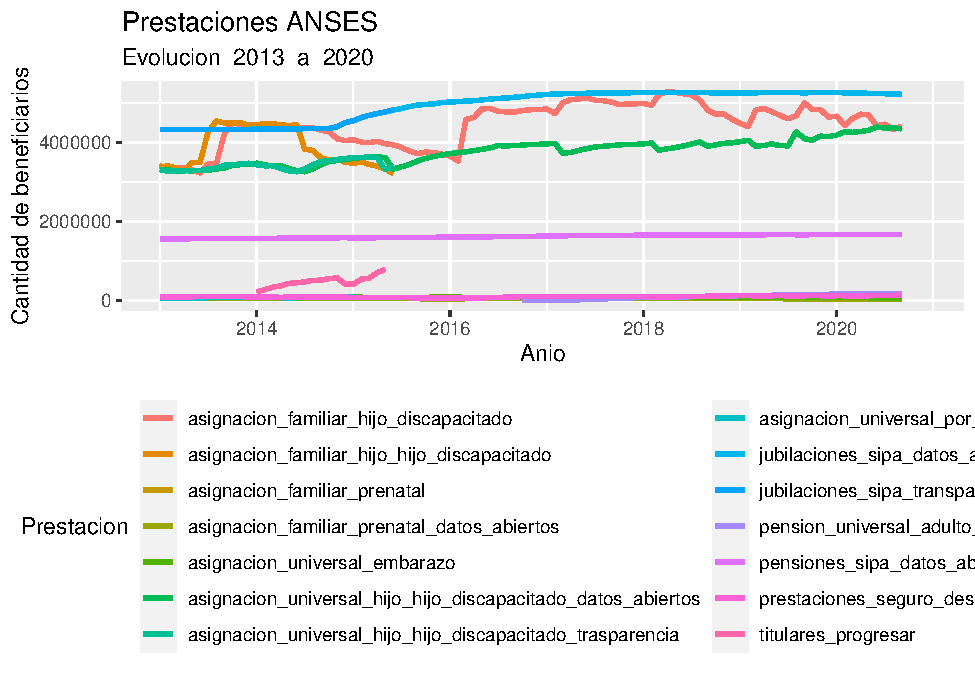
\includegraphics{Grupo4_Final_files/figure-latex/grafico_prestaciones_desagredadas-1.pdf}

Aislamos las prestaciones de las que se compone la AUH. La categoría
``otra condición'' es sin dudas la que hegemoniza el listado.

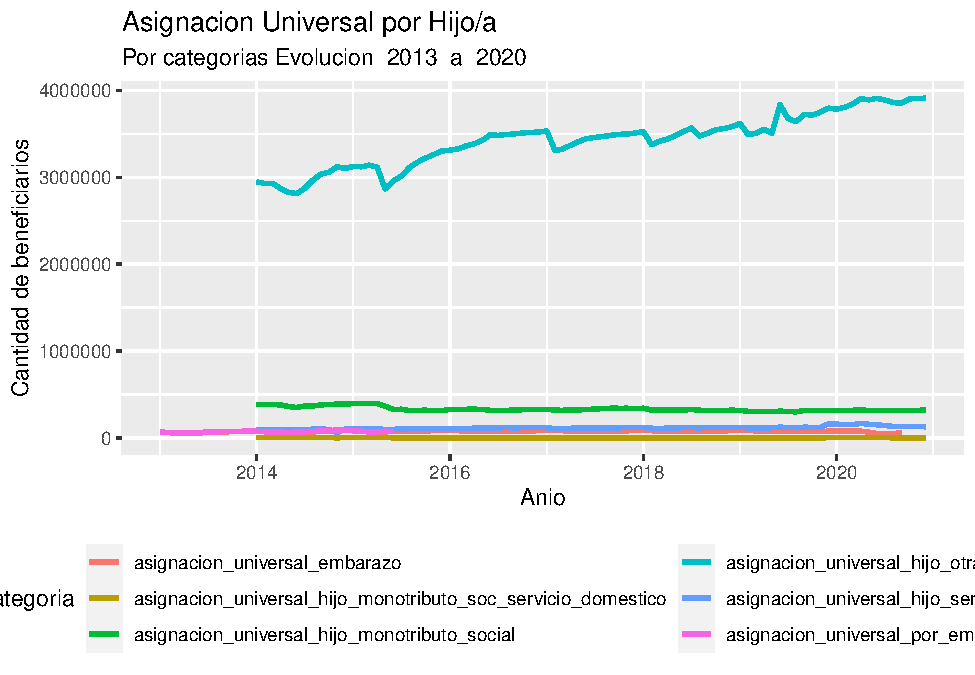
\includegraphics{Grupo4_Final_files/figure-latex/datos_prestaciones_auh-1.pdf}

Vemos el mismo gráfico pero normalizando por el total de la población
total de las edades objetivo. Se puede apreciar un crecimiento
importante entre los años 2015 y 2020.

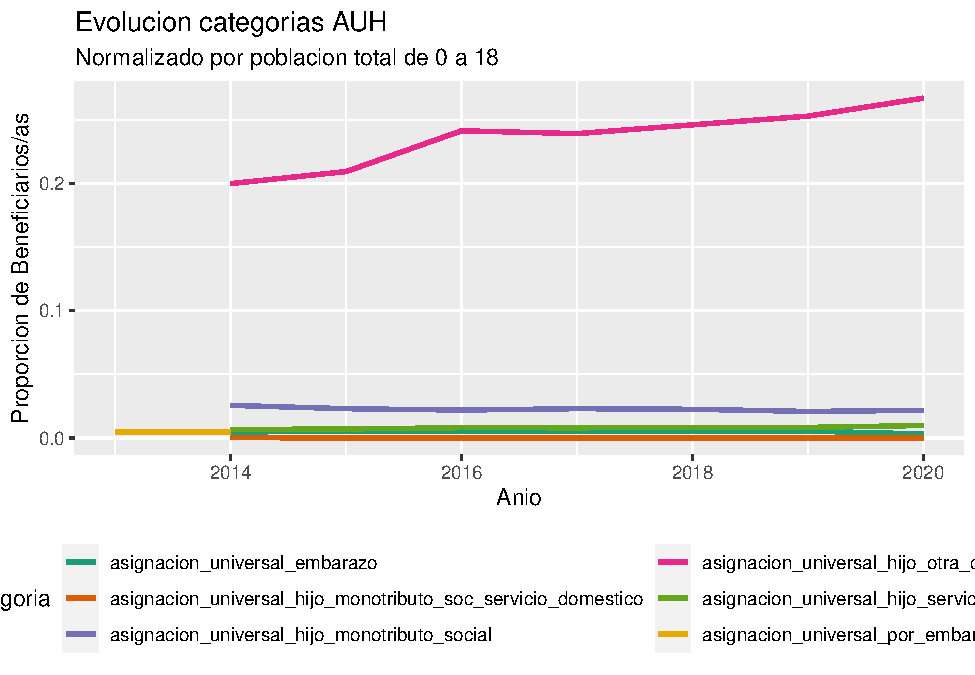
\includegraphics{Grupo4_Final_files/figure-latex/grafico_prestaciones_proporcion-1.pdf}

Analizamos una correlación negativa entre asignaciones familiares y
asignación por hijo. Interpretamos que esto es producto del deterioro de
las condiciones laborales durante los años de crisis económica que
expulsan a la fuerza de trabajo del mercado formal.

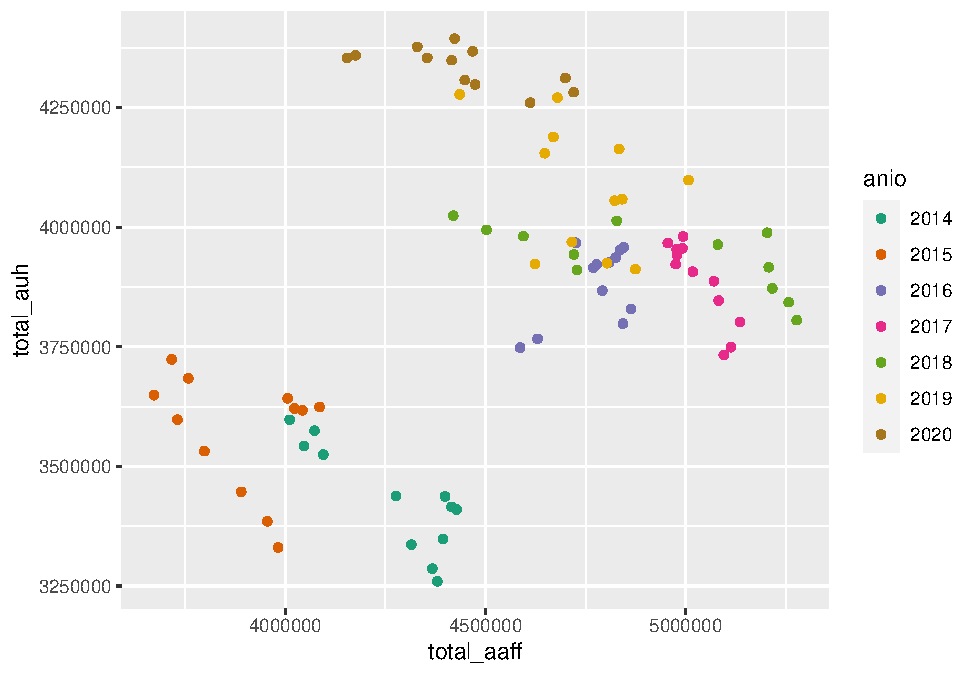
\includegraphics{Grupo4_Final_files/figure-latex/grafico_correlacion_auh_aaff-1.pdf}

Para descontar las distorsiones por el crecimiento poblacional
transformamos los valores en proporciones de los niños y niñas de acada
momento.

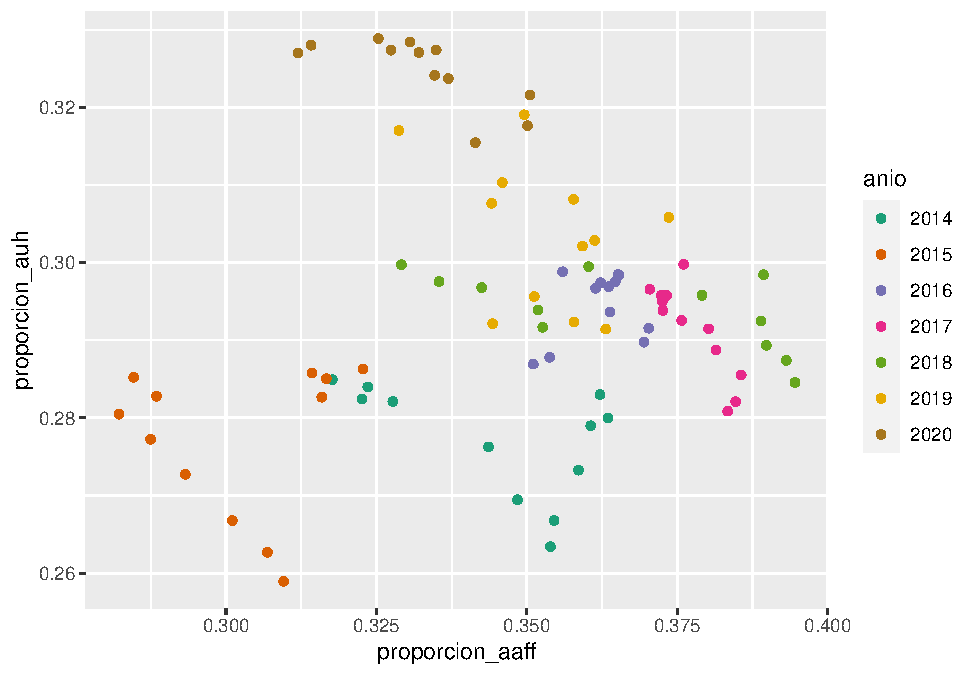
\includegraphics{Grupo4_Final_files/figure-latex/grafico_correlacion_auh_aaff_proporcion-1.pdf}

A continuación analizamos la evolución de la cantidad de hijos/as por
titular de la AUH. En contraposición con ciertas creencias, vemos que
más de la mayoría de las personas tienen un solo hijo/a. Y que esa
proporción no solo no baja sino que crece. A principio de la serie la
proporción de titulares con un hijo/a es del 49.48\% mientras que al
final pasó a 51.8\%. Por el contrario la proporción de 5 beneficiarios
por familia pasó del 2.92\% al 2.24\%.

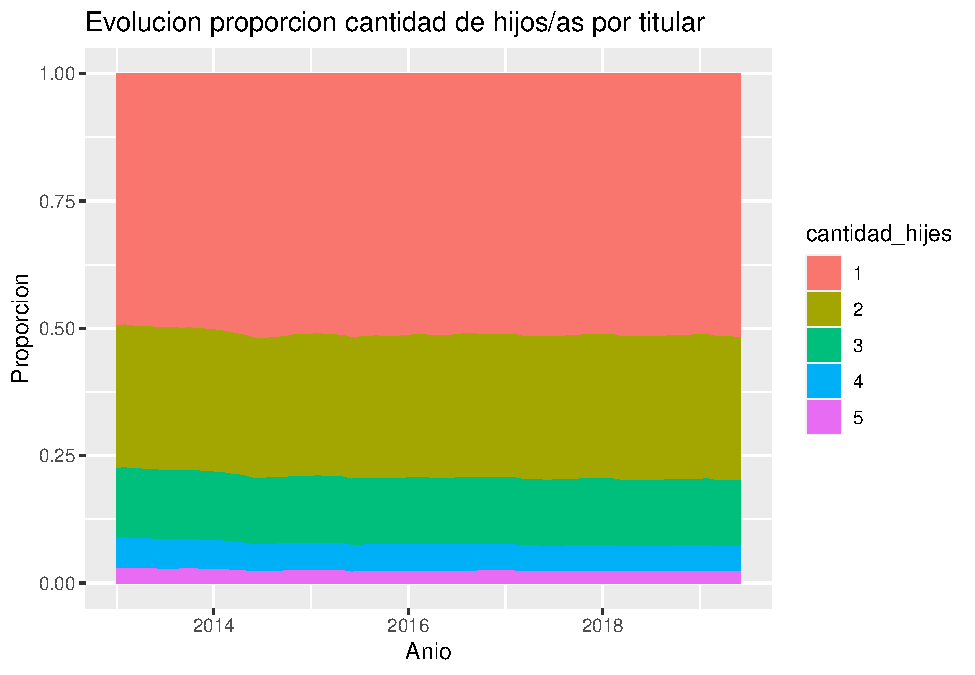
\includegraphics{Grupo4_Final_files/figure-latex/grafico_prestaciones_por_familia-1.pdf}

Deteniéndonos en la estructura de las edades de las/os titulares,
resulta interesante observar la evolución de la forma del gráfico. En
los primeros años se puede apreciar cierta similaridad en el segundo,
tercer y cuarto rango (20-25 , 25-30, y 30-35 respectivamente). Sin
embargo en los últimos años aparece una forma más bien triangular con un
pico en el rango de 25 a 30 años. Considerando que el total de
prestaciones viene en aumento, podría estar expresando que las madres
tienen sus hijos/as a edades mayores.

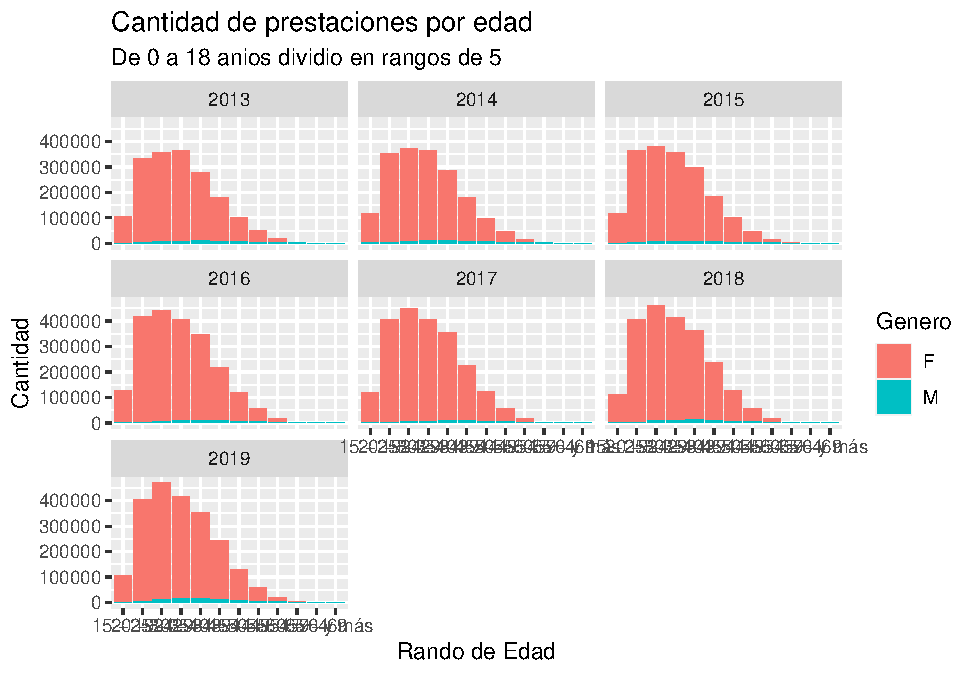
\includegraphics{Grupo4_Final_files/figure-latex/grafico_prestaciones_edad-1.pdf}

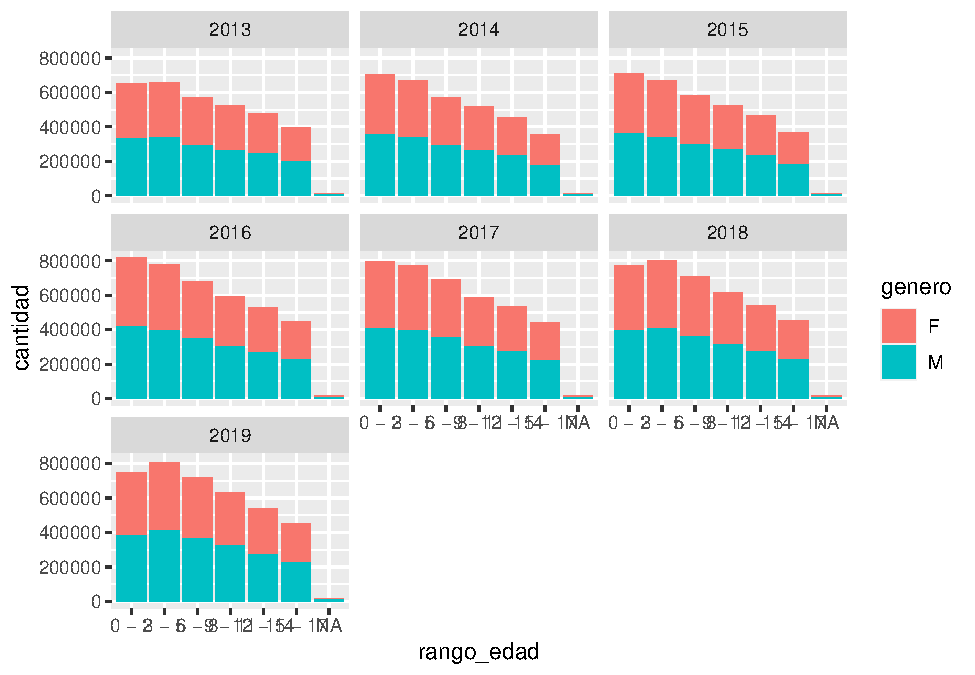
\includegraphics{Grupo4_Final_files/figure-latex/grafico_prestaciones_sexo_edad_ninies-1.pdf}

\hypertarget{conclusiones-y-reflexiones}{%
\subsection{\texorpdfstring{\textcolor{darkblue}{CONCLUSIONES Y
REFLEXIONES}}{CONCLUSIONES Y REFLEXIONES}}\label{conclusiones-y-reflexiones}}

Después del análisis de la implementación de esta política pública
podemos observar lo que hoy en día significa; lo que nació como una
ayuda de emergencia se ha trasformado en una ayuda indispensable para la
población más vulnerable o con menores posibilidades de generar ingresos
significativos para prescindir de ella. Contrariamente a lo ideado, el
grupo de beneficiarios activos es inferior al de pasivos, y la
diferencia crece en lugar de reducirse. Actualmente hay una correlación
inversa a la deseada en su nacimiento.

Con la implementación de la AUH se esperaba que en el futuro vaya
decreciendo el número de beneficiarios de AUH, ya que desde el Estado
Nacional se implementan otras políticas públicas activas para combatir
el trabajo no registrado lo que llevarían a reducir la población
objetivo del programa. Sin embargo, las condiciones económico --
sociales en el contexto histórico no parecen permitir que lo esperable
se haya transformado en un hecho, sino que, por el contrario, se deba
pensar en incrementar el prepuesto asignado año a año.

También podemos deducir que esta asignación es mal percibida por parte
de la población. Popularmente se cree que las mujeres que tienen bajos
ingresos informales, tienen hijos intencionalmente para cobrar la AUH y
que el monto total por 5 hijos es el mayormente cobrado. Después del
análisis de valores destinados de AUH se puede observar que el mayor
grupo poblacional que lo percibe es el compuesto por 1 y 2 hijos
desmitificando que se tienen 5 hijos para cobrar la AUH. Por otra parte,
el rango de beneficiarios que tiene 5 hijos fue disminuyendo con el
correr de los años. Este límite del quinto hijo nos plantea una
inquietud sobre la inclusión del sexto hijo en una futura actualización
de la normativa vigente para que el principio de universalidad sea más
elevado en la aplicación del beneficio.

Otra observación que quiebra la universalidad es que los trabajadores
que tienen ingresos familiares superiores a \$ 200.000, dejan de cobrar
asignación por hijo. Si bien se puede pensar que no lo necesitan porque
su ingreso es suficiente para la educación y protección de sus hijos; el
monto no parece ser tan elevado, pero se considera suficiente para
quedar excluidos. Asimismo, podemos considerar que este grupo paga
impuesto a las ganancias y que por lo tanto pueden deducir de la
liquidación de su impuesto, a sus hijos por un monto similar al de las
asignaciones por hijo.

Finalmente podemos concluir que esta política social ha causado un
impacto positivo con su implementación al punto de transformarse en un
beneficio muy difícil de cancelar en el futuro, no solo porque
transfiere fondo en forma directa y permanente a las familias más
vulnerables de la sociedad sino también, porque promueve la inserción en
el sistema de salud e incentivar la escolaridad, asegurando así la
inclusión y protección de derechos para todos los niños beneficiarios.

\end{document}
